\subsection{Redundancy Checker}
\label{sec:redundant}

\subsubsection{Design overview}
To check whether there is redundant computation across different iterations
of one loop instance or across different instances of one static loop, we need
to address several challenges.

\begin{figure}
  \centering
  \lstset{basicstyle=\ttfamily\fontsize{8}{8}\selectfont,
     morekeywords={+},keepspaces=true}
  \mbox{\lstinputlisting[mathescape,boxpos=t]{figures/Apache34464.c}}
  \caption{A cross-loop redundant bug in Apache}
  \label{fig:Apache34464}
\end{figure}

\emph{How to judge redundancy between two iterations/loop-instances?}
Given two iterations (or loop-instances) $i_1$ and $i_2$, since they have 
the same source code, 
a naive, yet expensive, solution is to record and compare the return value of
every memory read conducted by $i_1$ and $i_2$. Two better alternative
solutions are to record and compare only the values written by the
side-effect instructions, such as 
line 9 in Figure~\ref{fig:Mozilla477564},
or read by 
the source instructions\footnote{We define source instructions in a code
region $r$ as a set of memory-read instructions that side-effect
instructions in $r$ depend on and do not depend on any other instructions
inside $r$.}, 
such as source[i] at line 12 of Figure~\ref{fig:Apache34464}.

Among the the above two potential solutions, our design chooses the second one,
because it is
more informative for performance diagnosis 
to track the cause rather than the effect.

\emph{How to handle partial redundancy?}
In practice, redundant loops may be doing largely the same, but not exactly
the same, computation across iterations or loop instances. 
%It is also possible
%TODO define loop instance.
%that only some, instead of all, iterations in a loop are doing redundant
%computation. 
We will discuss how we handle this issue in Section \ref{sec:cal}.



\emph{How to lower the overhead of record-and-compare?}
Even if we only record and compare the values returned by source instructions
the run-time overhead and the log size
could still be large. We will use static analysis and run-time sampling
to lower this time and spatial
overhead 
(Section \ref{sec:inst} and \ref{sec:perf}).
%TODO static analysis alone is not sufficient, because some redundant is
%workload dependent

\emph{How to provide the most suitable fix-strategy suggestion?}
Finally, as discussed in Section \ref{sec:study_ob} and Table \ref{tab:root},
memoization and batching are both common fix strategies for redundant loops.
To pick the right fix strategies,
extra analysis is conducted by \Tool and presented in 
Section \ref{sec:redundant_fix}.

\subsubsection{Identifying source instructions}
\label{sec:dependence}

Informally, we use static analysis to identify a set of 
memory-read instructions that the loop computation depends on. We refer
to these instructions as \textit{source} instructions. The values returned
from them at run-time will be tracked and compared to identify
redundant computation.

Specifically, we first identify side-effect instructions in the loop, as 
discussed in Section \ref{sec:s_workless}; we then conduct static slicing 
from these instructions, considering both control and data
dependency, to identify source instructions.

%TODO How do you handle constant values? I didn't get it.
Our slicing ends when it reaches either a local-variable read conducted
outside the loop or a heap/global-variable read anywhere in the program.
For the latter case, our slicing stops because tracking data-dependency
through heap/global variables is complicated in multi-threaded C/C++
programs. For the former case, 
not including local-variable reads inside the loop can help reduce the
amount of data that needs to be recorded. 
When there are function calls inside the loop,  
we conduct slicing for return values of callees and side-effect instructions
inside callees. 
%In order to reduce the number of memory read we need to record inside callees, 
%we calculate previous writes conducted to the same address for each local-structure read and local-array read. 
%Since local structures and local arrays are mainly used in the declared functions, 
%it is easy to know whether read or write conducted on them are applied to the same address. 
We omit encountered constant values through slicing, because constant values will not influence whether a loop or an iteration is redundant. 


%We conduct slicing to for return values of callees and side-effect instructions
%inside callees. In order to reduce the number of memory read we need to record, 
%we design a GEN-KILL based algorithm to analyze previous writes for read from local structures and arrays 
%inside callees.
%TODO Linhai, I have no idea what you are talking about below
%For a memory read inside a callee function, 
%if its source is a structure or an array declared in the same function, 
%we use a GEN-KILL based algorithm to analyze previous writes for these reads. 
%We do not track previous writes for other memory reads, because it is very difficult to do inter-procedural alias analysis.  

% function() {
%  struct A;
%  A.a = 10;     // place a,
%  if(...)
%  {
%     A.a = 20;  // place b, value defined in place a will be killed, and this place gen a new value
%     print A.a  // A.a will be 20, because only value defined in place a is live 
%  }
%  return A.a;  // there will be memory read here. 
%  //We will do analysis to track where is the previous write for field a of struct A.
%  //The result will be write in place a, and place b
%  //We then conduct dependence analysis for these two writes.
%  //We only do this for read from structure and array declared in the same function. 
% }

The analysis for cross-iteration and cross-loop redundancy analysis is pretty
much the same. The only difference is that, if a memory read instruction 
$i$ in a loop depends on the value returned by instruction $j$ in an earlier
iteration, we stop tracing the dependence at $i$ and consider $i$ as a
source instruction for cross-iteration redundancy analysis, while we continue
the slicing for cross-loop redundancy analysis. 
For example, 
the instruction defining the value of \texttt{i} is the only side-effect instruction 
for the loop at line 12 of Figure~\ref{fig:Apache34464}. 
The source instructions calculated by cross-loop dependence analysis include 
memory read \texttt{source[i]} inside the loop, 
and three values defined outside the loop, 
which represent the initial value of \texttt{i}, the value of \texttt{max} and \texttt{first} respectively. 
In contrast, 
the source instructions calculated by cross-iteration dependence analysis 
include value \texttt{i} defined in previous iteration, 
memory read \texttt{source[i]}, 
and two values defined outside the loop (\texttt{max} and \texttt{first}).  


\comment{
We consider two types of dependence, control dependence and RAW data dependence. 
We build control dependence graph according to the algorithm discussed in~\cite{controldep}. 
If block A is one of ancestors of block B on the control dependence graph, 
we consider all instructions in block B control depend on the branch condition in block A. 
Data dependence is mainly calculated based on instructions' operands. 
We define several types of instrumentation sites. 
The inputs of our dependence analysis are instructions, 
and the output of our dependence analysis is a set of dependent values, 
including instrumentation sites and constant values. 

Before calculating dependence inside the monitored loop, 
we conduct inter-procedural dependence analysis for each function directly called by the loop. 
The formal parameters of each direct callee, memory instructions, 
including load, memcpy, and memmove, 
whose source is not from local structures or arrays, 
and return values of library function calls are instrumentation sites. 
During calculating dependence, 
we consider formal parameter data depend on all real parameter, 
the return value of each call site data depend on return inside the callee function, 
and all instructions inside one callee functions inherit control dependence of all its call site. 

If a direct callee from the monitored loop does not contain recursive function calls, 
we use a three-stage method to solve the infeasible path problem. 
Assume function A is called inside the monitored loop, function A will call function B, 
and function B will call function C. 
We will have a call tree A $\rightarrow$ B $\rightarrow$ C. 
This call tree does not have recursive function calls, so our three-stage method can apply to this case. 
At the first stage, we conduct intra-procedural dependence analysis for each function.  
We consider return values of all call sites as instrumentation sites. 
For example, we consider both the return value of B in A and the return value of C in B as instrumentation sites. 
At the second stage, we process each function bottom-up on the call tree. 
For each call site inside a function, we calculate 
how the return value depend on real parameters based on dependence information inside the callee.
Back to our example, we will process the three functions in order C, B, and A.
When processing function B, we calculate the dependence for the return value of function C 
based on the dependence information inside C and the real parameters of the call site.
At the last stage, we process each function top-down on call tree, 
and calculate dependence for instruction inside a callee function based on information from all its call site. 
At this stage, we will process the three function in the order A, B, and C. 
We update dependence information inside function B, according to control dependence and real parameters of its call site in A. 

We design a Gen-Kill based intra-procedural analysis to 
calculate which previous writes a memory read from local structures and arrays depends on. 
The basic idea is that a memory write will kill all previous writes whose destination address it can cover, 
and the memory write will generate a new write to its destination address. 
Each memory read depends on previous writes whose destination addresses overlap with its source address. 

For the monitored loop, we calculate dependent values for all site-effect instructions, 
including side-effect instructions inside the loop and side-effect instructions inside the callees. 
For cross-loop dependence analysis, instrumentation sites include values defined outside the loop, 
memory reads inside the loop, memory reads not from local structure and arrays inside callees, 
and return values of library function calls. 
For cross-iteration dependent analysis, instrumented sites also include value defined in previous iterations. 
For example, the instruction defining the value of \texttt{i} is the only side-effect instruction 
inside the loop at line 12 in Figure~\ref{fig:Apache34464}. 
After running cross-loop dependence analysis, the dependent values include 
memory read \texttt{source[i]} inside the loop, 
and three values defined outside the loop, 
which represent the initial value of \texttt{i}, the value of \texttt{max} and \texttt{first} respectively. 
After running cross-iteration dependence analysis, 
the dependent value include value \texttt{i} defined in previous iteration, 
memory read \texttt{source[i]}, 
and two values defined outside the loop (\texttt{max} and \texttt{first}).  

}

\subsubsection{Identifying redundant loops}
\label{sec:cal}

After identifying source instructions, we instrument them to record
what values they read from memory
at run time.
%Specifically, we will assign
%a unique ID for each source instruction, and a pair of $<InstID, Value>$
%will be recorded at run time with the execution of a source instruction.
Our trace also includes some delimiters and meta information that allows
trace analysis to differentiate values recorded from different instructions, 
loop
iterations, loop instances, and so on.
%TODO
%All values defined outside the loop is recorded in block O. 
%We record a delimiter, loop instance number and values defined in previous iterations in block H1'.
%Since we only consider redundant iterations from the same loop instance,  
%we do not record values defined outside the loop for cross-iteration redundancy. 



After collecting values returned by source instructions from every iteration
of one or multiple loop instances, we need to process the trace and decide
whether the loops under study contain cross-iteration redundancy or 
cross-loop redundancy. We will first present our high-level algorithms, followed
by the exact implementation in our prototype.

\paragraph{High-level algorithms}
For cross-iteration redundancy, we need to answer two questions. 
First, how to judge whether
two iterations are doing redundant work?
Second, is a (dynamic) loop problematic when it contains only few 
iterations that are
redundant with each other?

Our answer to these two questions stick to one principle: there should be
sufficient amount of redundant computation to make a loop likely root-cause
for a user-perceived performance problem and to make itself worthwhile to
get optimized by the developers. Consequently,
for the first question, \Tool takes a strict 
definition --- only iterations that are doing exactly the same computation are
considered redundant. Since one iteration may not contain too much computation,
a weaker definition here may lead to many false positives. For the 
second question, we believe there should be a threshold. In our current 
prototype,
when the number of distinct iterations is less than half of the total iterations, 
we consider the loop to be cross-iteration redundant. 
%when the number of distinct iterations is less than half of the total iterations 
%iterations/(distinct iterations) = 2

\begin{figure}
  \centering
  \lstset{basicstyle=\ttfamily\fontsize{8}{8}\selectfont,
     morekeywords={+},keepspaces=true}
  \mbox{\lstinputlisting[mathescape,boxpos=t]{figures/Apache37184.java}}
  \caption{A cross-iteration redundant bug in Apache}
  \label{fig:Apache37184}
\end{figure}

For example, Figure~\ref{fig:Apache37184} shows a loop from Apache-Ant that
contains cross-iteration redundancy.
Under the problem triggering input, there are
only few distinct listeners, and most of the
loop iterations in \texttt{fireMessageLoggedEvent}
are doing redundant work. 
%The problem for this bug is that developers say that the performance 
%loss happens in fireMessageLoggedEvent, but in the code I found, function
%messageLogged does not contain anything, and it is an empty function.
%I guess either developers do not have correct understanding of this bug,
%or I did not find the correct codes. 





For cross-loop redundancy, we need to answer similar questions,
especially how to judge whether two loop instances are doing redundant work ---
should they contain exactly the same number of iterations and doing exactly
the same computation in each iteration?
%Second, is a (static) loop problematic when it contains two instances that
%are redundant with each other?

Our answers here are different from our answers above for cross-iteration
redundancy analysis.
We do not require two loop instances to
conduct exactly the same computation to be considered redundant. The rationale
is that a whole loop instance contains a lot of computation, much more than
one iteration in general. Even if only part of its computation
is redundant, it could still be the root-cause of a user-perceived performance
problem and worth developers' attention. 

In fact, in practice, we almost have never seen cases where different loop 
instances are doing exactly the same computation.
For example, Figure~\ref{fig:Mozilla477564} demonstrates a cross-loop redundancy
problem in Mozilla. Here, the
latter instances contain more iterations than previous instances. 
Figure~\ref{fig:Apache34464} shows an example in Apache, 
The inner loop, which starts from line 9,  
searches from the beginning of a string \texttt{sb} for a target sub-string 
\texttt{s}. Since the outer loop, which starts on line 36, appends one 
character to \texttt{sb} in every iteration, every inner loop instance is 
doing computation that is similar, but not exactly the same, 
from its previous instance.


\paragraph{Detailed algorithm implementation}

The implementation of checking cross-iteration redundancy is straightforward.
We will record a sequence of $<InstID, Value>$ pair for every monitored
iteration, with each $InstID$ representing a unique source instruction.
We consider two iterations to be redundant, if their sequences are exactly the
same. To make sure a loop contains sufficient redundant computation, 
we calculate a loop's \textit{cross-iteration redundancy rate} --- dividing 
the total number of iterations in the loop by the number of distinct iterations.
The smaller the rate is, with 1 being the minimum possible value, 
the less cross-iteration redundancy the loop contains.

The implementation of checking cross-loop redundancy goes through several
steps. First, for $k$ dynamic instances of a static loop $L$ that appear
at run time, denoted as $l_1$, $l_2$,
..., $l_k$, we check whether redundancy exists between $l_1$ and $l_2$, 
$l_2$ and $l_3$, and so on. Second, we compute a 
\textit{cross-loop redundancy rate} for $L$
--- dividing the number of redundant pairs by $k-1$.
The smaller the rate is, with 0 being the minimum possible value, the
less cross-loop redundancy $L$ contains.
Here we only check redundancy between consecutive loop instances, because  
checking the redundancy between every pairs of loop
instances is time consuming.

The key of this implementation is
to judge whether two dynamic loop instances $l_1$ and $l_2$ 
are redundant or not.
The challenge is that $l_1$ and $l_2$ may have executed different number of
iterations; in different iteration, a different set of source instructions
may have executed. Therefore, we cannot simply merge values from different
source instructions and iterations together and compare two big data sequence.
Instead, we decide to check the redundancy for each source instruction across
$l_1$ and $l_2$ first, and then use the average \textit{redundancy rate} of
all source instructions as the \textit{cross-loop redundancy rate} between
$l_1$ and $l_2$. 

We calculate the redundancy for one source instruction $I$ by normalizing the
edit-distance between the two sequences of values returned by $I$ in the two
loop instances. The exact formula is the following:

%\[
%\Scale[0.8]{
%min\_dist(SeqA, SeqB) = min(dist(SeqA,SeqB), r\_dist(SeqA, SeqB))
%}
%\]

\[
\Scale[0.8]{
	Redundancy(I) =  \frac{dist(SeqA,SeqB) - (len(SeqA) - len(SeqB))}{len(SeqB)}
}
\]

Here, $SeqA$ and $SeqB$ represent the two value sequences corresponding to $I$
from two loop instances, with $SeqA$ being the longer sequence.
$dist$ means edit distance, and $len$ means the length of a value sequence.
Since the edit distance is at least the length-difference between the
two sequences and at most the length of the longer sequence, we use the 
subtraction and division shown in the formula above to normalize the
redundancy value.

%$r\_dist$ means edit distance after 
%we reverse one sequence. 

%TODO
%We define two configurable thresholds to filter out instance pairs which are both too short, 
%or one is too short compared with the other one.

%TODO
%It is also possible that a source instruction is executed outside the loop.
%We divide values defined outside the loop into several cases.
%Firstly, the value defined outside the loop is only used in the first iteration, 
%and all related values used in following iterations have already been recorded, 
%like the initial value of variable \texttt{n} in Figure~\ref{fig:Mozilla477564}. 
%We omit values defined outside the loop like this.
%Secondly, the value defined outside the loop represent the initial value of an induction variable, 
%like the initial value of variable \texttt{i} in Figure~\ref{fig:Apache34464} 
%for the loop at line 12. We deduce the value sequence of the induction variable 
%based on its initial value and stride, and compare the calculated sequences. 
%Thirdly, the value defined outside the loop only influences side-effect instruction through control dependence, 
%and variables it compares with is not calculated from memory read, 
%like variable \texttt{max} in Figure~\ref{fig:Apache34464}. We think that this type of values only influence how many iterations the loop will execute.
%We calculate redundancy for this type of values by dividing the smaller variable value with the larger one. 
%For all other cases, when the values from two compared instances are the same, redundancy is 1, otherwise, redundancy is 0.

\subsubsection{Dynamic performance optimization: sampling}
\label{sec:inst}

%\begin{figure}[ht]
%\center
%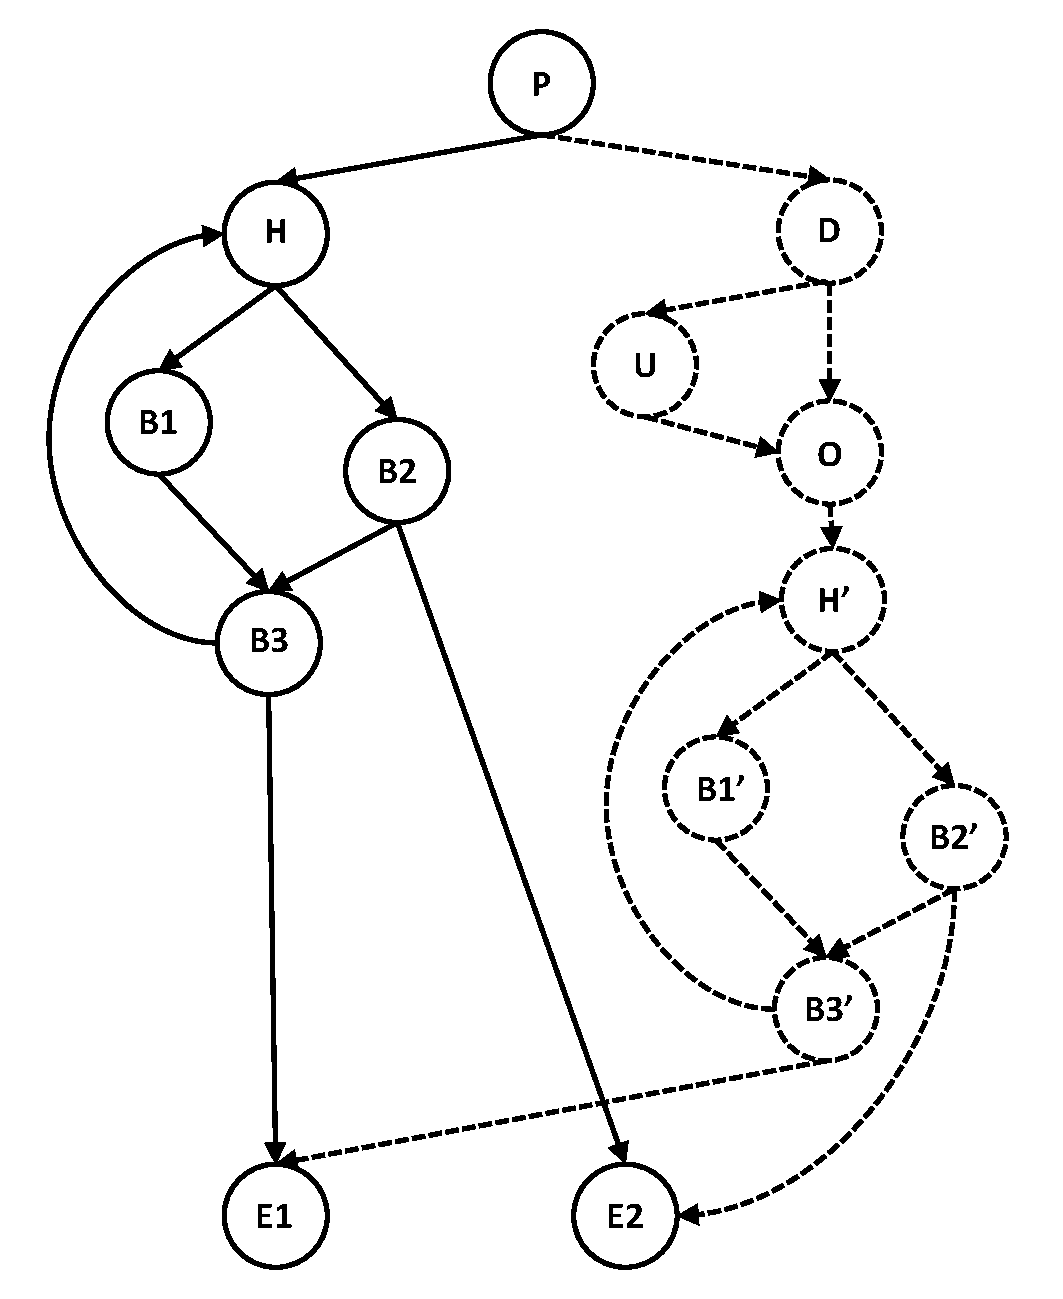
\includegraphics[width=0.7\linewidth]{figures/CL-I}
%\caption{Cross-loop Instrumentation}
%\label{fig:CL-I}
%\end{figure}

Recording values returned by every source instructions would lead to 
huge run-time time. To lower the overhead,
we use random sampling to reduce the number of instructions that we
track at run time. Due to the repetitive nature of performance bugs,
we will still be able to recognize redundant 
computation as long as the sampling rate is not too sparse (we will evaluate
this in Section \ref{sec:experiment}). 
Our sampling scheme requires almost no changes to our redundancy 
identification algorithm discussed in Section \ref{sec:cal}.


%Another observation, which can also be demonstrated by examples shown in Figure~\ref{fig:Mozilla477564} and Figure~\ref{fig:Apache34464}, 
%is that two consecutive loop instances are good targets to compare.

%There are two possible reasons for cross-iteration redundancy. 
%The first one is loop-invariant computation, which can be identified statically, 
%and it is the target for traditional compiler optimization. 
%The second one is repetitive processed elements, like GCC\#27733 shown in Figure~\ref{fig:GCC27733}. 
%When processed elements are repetitive, the computation conducted by different iterations is exactly the same. 
%If we compare a pair of iterations, we may fail to observe redundancy. 
%For cross-iteration redundancy, we randomly sample iterations, 
%and compare distinct computation number with the total number of sampled iterations. 

\paragraph{Cross-iteration redundancy analysis}
Our high-level sampling strategy is straightforward:
randomly decide at the
beginning of every iteration whether to track the values returned by
source instructions in this iteration.

The implementation is similar with previous sampling work 
\cite{liblit03,liblit05}.
Specifically, we create a clone of the original
loop iteration code, including functions called by the loop directly or
indirectly, and insert value-recording instructions along the
cloned copy. 
We then insert a code snippet that conducts random decision to
the beginning of a loop iteration. 
Two variables \texttt{CurrentID}, which is initialized as 0, 
and \texttt{NextSampleID}, which is initialized by a random integer, 
are maintained
in this code snippet. \texttt{CurrentID} is increased by 1
for each iteration. When it matches \texttt{NextSampleID}, the control
flow jumps to the value-recording clone of the loop iteration and the 
\texttt{NextSampleID} is increased by a random value. Different sampling
sparsity setting will determine the range from which the random value is
generated.

%\begin{figure}
%\center
%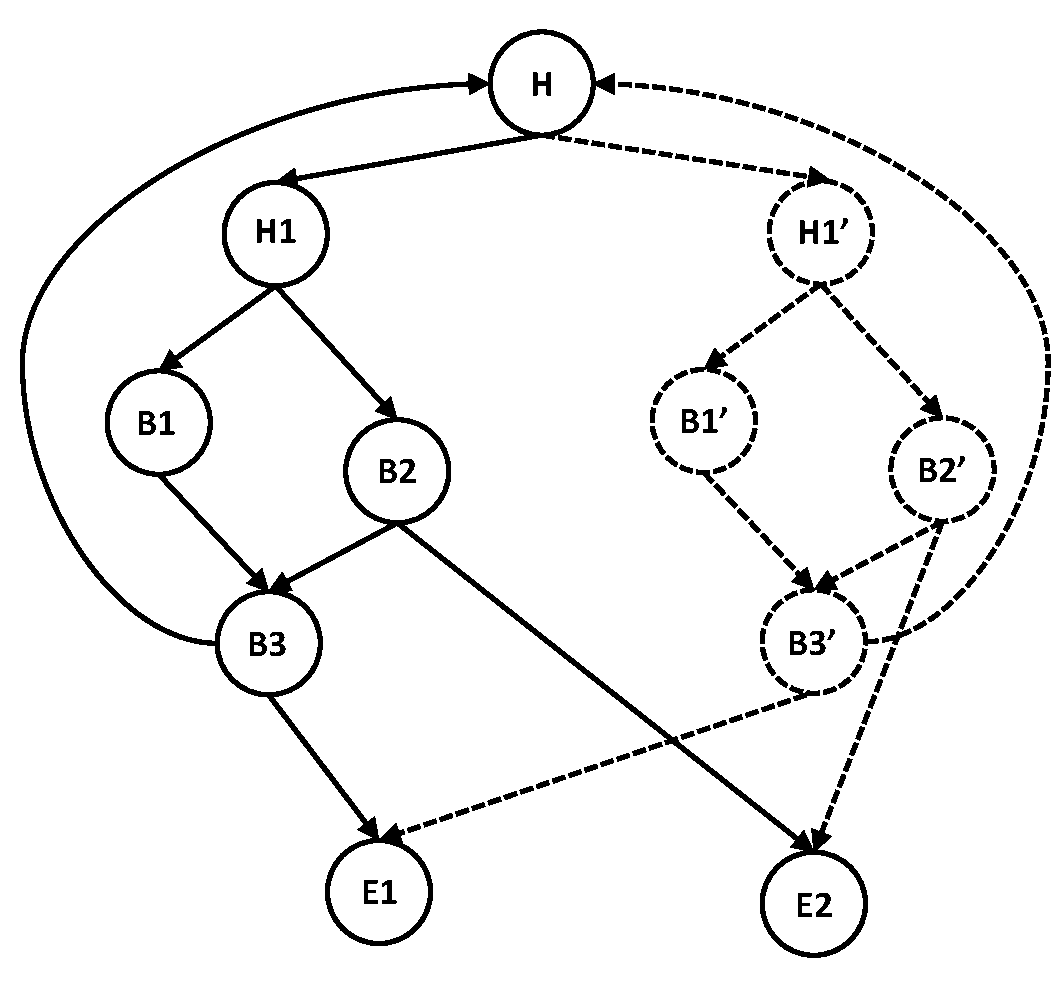
\includegraphics[width=0.7\linewidth]{figures/CI-I}
%\caption{Cross-iteration Instrumentation}
%\label{fig:CI-I}
%\end{figure}

\paragraph{Cross-loop redundancy analysis} 
At high level, we randomly decide at the beginning
of every loop instance whether to track values for this instance. 
Since we will need to compare two consecutive loop
instances for redundancy, once we decide to sample one loop instance, we will
make sure to sample the immediately next loop instance too.
The implementation is straightforward by cloning the whole loop and making
sampling decisions in the loop pre-headers.
%; (2)
%sampling is conducted when \texttt{CurrentID} equals either
%\texttt{NextSampleID} or \texttt{NextSampleID}$+1$, with \texttt{NextSampleID}
%increased by a random value in the latter case.

%TODO
%For each monitored memmove or memcpy instruction, 
%we record its ID, the length of accessed memory, 
%and the content of the accessed memory. 



%\paragraph{Handling recursive functions}
%We also conduct sampling to our redundancy analysis for recursive functions.
%For a recursive function, we first create an instrumented clone copy of 
%the whole function body.
%We then add a sampling-control code snippet at the entry point of the function,
%where \texttt{CurrentID} and \texttt{NextSampleID} are maintained to decide
%whether to execute the original function body or the instrumented 
%value-recording clone copy.
%We also create clones for all the callee functions of the recursive function
%under study, so that the sampling decision can be correctly conducted
%throughout the call chain.

\subsubsection{Static analysis for performance optimization}
\label{sec:perf}

We conduct a series of static analysis to reduce the number of instructions we 
need to monitor. 

First, we identify and avoid monitoring memory reads whose return values can be 
statically proved to
not change throughout one loop instance (i.e., for cross-iteration
redundancy analysis) or multiple loop instances (i.e., for cross-loop redundancy
analysis). Since we implement \Tool at LLVM byte-code level, a major part of this
analysis is already done by LLVM, which lifts loop-invariant memory
accesses out of loops. The only extra analysis we did is to 
prune memory reads whose reading address is loop invariant, and there are no writes 
inside the loop which are possibly conducted on the same address. 
For example, the read address of \texttt{aNode.localName} and \texttt{aNode.namespaceURI}
in Figure~\ref{fig:Mozilla347306} is loop-invariant, and there are no write conducted 
on the same address. We do not need to record these two memory read. 
%It is easy to lift read from local variable outside the loop. 
%Compiler is conservative to move read, which may cause exception, outside the loop.
%I think this part of analysis is to prune memory read which is invariant, but unsafe to be moved out by compiler. 
%llvm is very conservative to move memory read from array/structure/global variable/heap variable
%outside the loop.
%what we do is if the read address is loop invariant, and there are no other write possibly 
%write to the same place, we will not record the memory read.

%TODO: Linhai, I don't understand your original writing. Pls rephrase, and provide
%an toy example.
%For each monitored memory read, we use loop-invariant analysis to identify 
%whether the read address is loop-invariant. 
%If the address is invariant, and there are no memory writes whose addresses 
%may/must alias to the read address, we will not instrument the memory read.

%ANSWER:
%while(i=lower[j]; a[i]<100 & i<upper[j]; i++); 
%The memory read upper[j] is conducted in each iteration.
%The read address upper+j is loop-invariant. If there is not write to the same
%address, the read is also loop-invariant, and we do not need to record the memory read.
%we conduct alias analysis, and analysis whether there are memory writes, whose
%address may/must alias to the read address. 

Second, we identify and avoid monitoring some memory reads whose return values 
can be statically proved to be different throughout one loop instance in 
cross-iteration redundancy analysis.
Specifically, for read on loop induction variable, such as i for loop at line 12 of Figure~\ref{fig:Apache34464}, 
%Specifically, reading of loop induction 
%variables, such as XXX, are always identified as source instructions in % variable i for loop at line 12
%cross-iteration redundancy analysis; 
we also know for sure that their return
values are different in different iterations. 
If source instructions include read on loop induction variables, we know that 
there could not be cross-iteration redundancy. 
We use scalar evolution analysis
provided by LLVM to identify induction variables and avoid tracking their
values.
%induction variables are not always identified as source instructions.
%it could be possible that side-effect instructions do not depend on induction variables.
%for example, side-effect instruction may only depend on array content, and array index 
%will not be source instructions

%TODO: Linhai, I find it hard to believe that consider "there will not be
%cross-iteration redundancy simply because induction variable is in the 
%dependent set. Really? The input workload itself could be repetitive, and hence
%could still deserve monitoring, right? 
%


%ANSWER: this is true according to how we calculate cross-iteration redundancy.
%We only consider iteration from the same loop instance.
%induction variable will be changed in each iteration by a fix constant, so
%the value of induction variable will be different from each other in each iteration of the same loop instance. 
%The case you mention is 
%for(i=0; i < 10; i ++) {
%  c = A[i]; 
%   ...   // all other computation only depend on c        
% }
%Our dependence analysis will report the memory read A[i] as dependent value, not i.
%If the content of A is repetitive, we will identify cross-iteration redundancy.
 
%For cross-iteration instrumentation, we use scalar evolution analysis to identify 
%whether there are induction variables in the dependent value set. 
%A induction variable will be increased or decreased by a fix amount in each loop iteration. 
%If there are induction variable inside the dependent value set, 
%we know that there will not be cross-iteration redundancy. 


Third, sometimes we only record the memory-address range of a sequence of memory
read, instead of the value returned by every read, in cross-loop redundancy
analysis. 
The loop at line 12 in Figure~\ref{fig:Apache34464} shows an example.
The content of array \texttt{source} is never modified
throughout the outer-loop, which starts 
at line 12 in the Figure~\ref{fig:Apache34464}.
%We do not have the static analysis to prove the content of array does not change.
%for source[i] for the loop at line 12, we only need to record source, initial value of i and final value of i. 
%TODO
%Do you really do analysis to prove that the source array is not changed?
%ANSWER
%Shan, I do not have invariant analysis to prove the the source array is not changed.
%I remove that part of writing in the last version I sent to you. 
%It is very difficult to implement the invariant analysis.
%I plan to discuss this in limitation part of this section, and say that this could bring false positives.
%There are reasons why I feel it is too difficult to implement the invariant analysis:
%1. it is difficult to find the range (the outer loop) to apply the analysis.
%assume we have loopA, loopB and loopC. loopA contains loopB, and loopB contains loopC. 
%we are analyzing loopC. It could be possible that loopB only execute 1 or 2 iterations, and loopA is the real outer loop
%2. It is very difficult to prove that there is no other loop inside the outer loop which does not write to the same array.
%There could be cases like:
% for(i = 0; i < 10; i++)
%   func(&(A[i]));
% func will write to its parameter.
Therefore, to check whether different inner loop instances read similar
sequence of array data, we only need to record the starting and 
ending array index touched by each inner loop, significantly reduce the 
monitoring overhead. To accomplish this optimization, we again leverage
the scalar evolution analysis provided by LLVM. The scalar evolution analysis
tells us whether the address of a memory read instruction
is a loop induction variable. For example, the address for memory read \texttt{source[i]} is added by one in each loop iteration,
so it is a loop induction variable. 
From the scalar evolution analysis, we know that the starting address is \texttt{source} plus the initial value of \texttt{i}, and the ending address
is source plus the ending value of \texttt{i}.  
%TODO Linhai, I don't understand your original text. The address is 
%source+i; loop induction variable is i. What do you mean by "the read address
%is an induction variable"? Please rewrite.

%ANSWER
%Shan, both source + i and i are induction variables, because both of them 
%will be added by 1 in each iteration. The only difference between these two 
%are their initial values.
%For cross-loop redundant bugs, we also rely on scalar evolution analysis to identify whether the read address
%is an induction variable for each monitored read instruction. 


\subsubsection{Fix strategy recommendation}
\label{sec:redundant_fix}
As discussed in Section \ref{sec:tax_study}, extra analysis is needed to
decide whether batching or memoization should be suggested to fix a 
loop that conducts redundant computation.

For cross-iteration redundancy, batching is often used towards
batching I/O related operations, based on our empirical study. 
Therefore, we treat I/O related redundancy separately.
Specifically, when the only side effect of a loop is I/O operations
and the same statement(s) is executed in every loop iteration, we report this
as I/O related redundancy problem and suggest batching as a potential fix
strategy. 

For cross-loop redundancy, whether to use memoization or batching often
depends on which strategy is cheaper to use. \Tool uses a simple
heuristic. If 
the side effect of each loop instance is to update 
a constant number of memory locations, like the 
buggy loop in Figure~\ref{fig:Mozilla477564} and Figure~\ref{fig:Apache34464}, 
we recommend memoization. Instead, if the side effect is updating 
an sequence of memory locations, with the number of locations increasing
with the workload, memoization is unlikely to help save much computation.

%we xxx
%TODO

%%if side effect of the loop is to define several scalar value used outside the loop, we recommend memoization.
%%if side effect is to write to distinct memory address or conduct system call, 
%%we recommend batch


